
\section{System Evaluation}
% \section{System Evaluation}
% write about cross validation results, within users and per-user models

We evaluated our system by running various cross-validation tests with usage data collected with 30 participants.
In this section, we describe the details of the validation process and result.
\subsection{Preprocessing Raw Data}
After analyzing the raw data, we found all pointing operations are performed on the right side of every \emph{touchpad frames}, because all of our participants are right-handed.
This user behavior indicates we can build our classifier, which enables automatic mode switching, with right half of raw images. 
So we used a 29x20 10-bit image instead of a 58x20 10-bit image as input data for our RDF classifier to speed up the classification process.
% write about the feature extraction method and why we choose to scale down the original image
% We first tried to build a classifier with MHIs generated with filtered 58x20 10-bit image, the recognition rate and result were both quite impressing.
% But the classifiers trained with higher resolution images were more sensitive with touched position, which requires too much training data, a 30-minute single user training data cannot generate a usable classifier.
% We then decided to build another classifier with down-scaled 29x10 10-bit image, it significantly reduced the amount of data required to build a working classifier.


\subsection{Testing Parameters}
%Final: reviewer要求number of tees, tree depth, split function
The forest size improves the performance of RDF classifier at a linear cost of time, to build a real-time interactive system, we set the number of trees to 50 and the maximum depth per tree to 25 for more accurate recognition. 
%Final:
%Also, the split function we used was default Weka[] straitfied cross validation, and the offset was not constraint.
% The maximum depth of RDF also affects the performance of the classifier.
% We conducted a experiment to determine the best value for recognizing user intention.
% We run a 5-fold cross validation with 30 frame referenced while building Motion Signature, maximum tree depth from 15 to 25.
% The experiment result is shown at Figure[X].
% We can see the over fitting start when maximum depth is [XX], so we set the maximum depth to [XX].
% \begin{figure}[!h]
% \centering
% 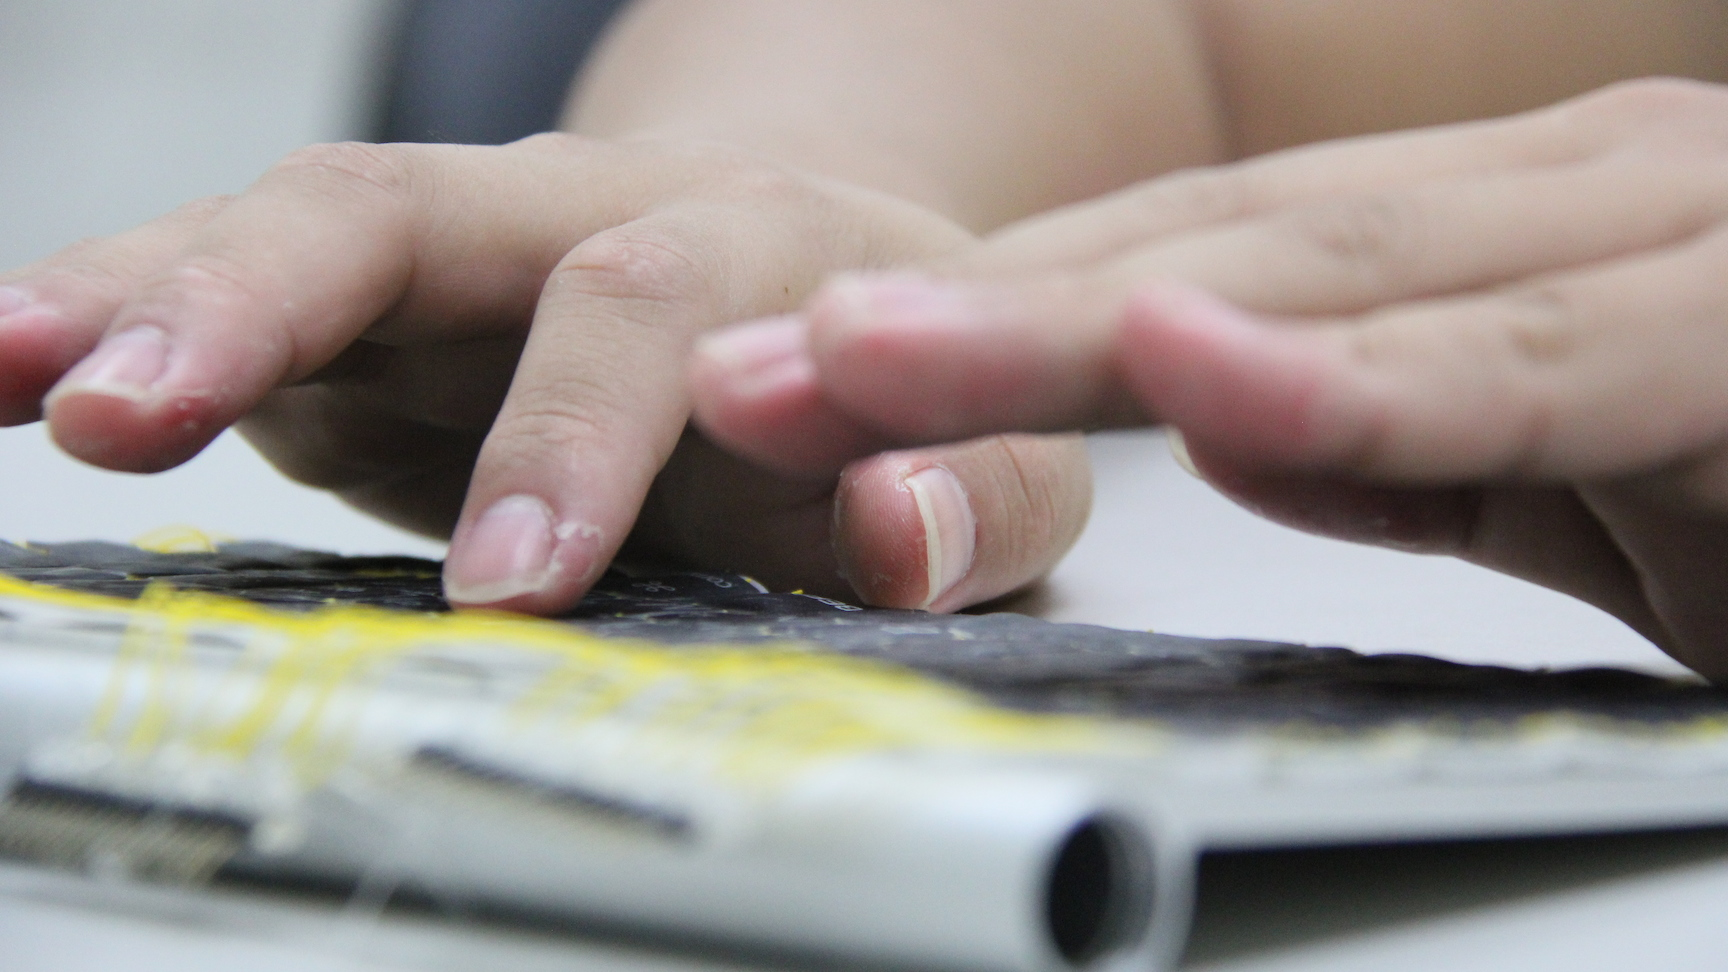
\includegraphics[width=0.8\columnwidth]{figures/figure4.png}
% \caption{Classification accuracy of 5-fold cross validation with 30 frame referenced while building Motion Signature. X axis is the maximum tree depth from 15 to 25. }
% \label{fig:figure4}
% \end{figure}
While running the experiments, we found the number of frames referenced while building Motion Signature ($N_{f}$) can strongly affect the performance for recognizing user intention, so we need to find out a good parameter for the number of frames referenced.
We run a 5-fold cross validation with 1-20 frames referenced. The results are shown in Figure~\ref{fig:figure3}.
We can find that the recognition rate is very low when $N_{f}$ is 1. Then gradually rising while $N_{f}$ is increasing.
The recognition rate stabilized around 98\% when $N_{f}$ = 30.
This means we only need to remember 30 frames to achieve a good recognition rate, and we can recognize the user's intention with about 2.3 seconds of previous surface action.
We found this parameter can have a great impact on the performance of the system, but previous work did not mention this. \cite{96bytes}
According to the result, we set $N_{f}$ = 30 in the following experiments.

\begin{figure}[!ht]
\centering
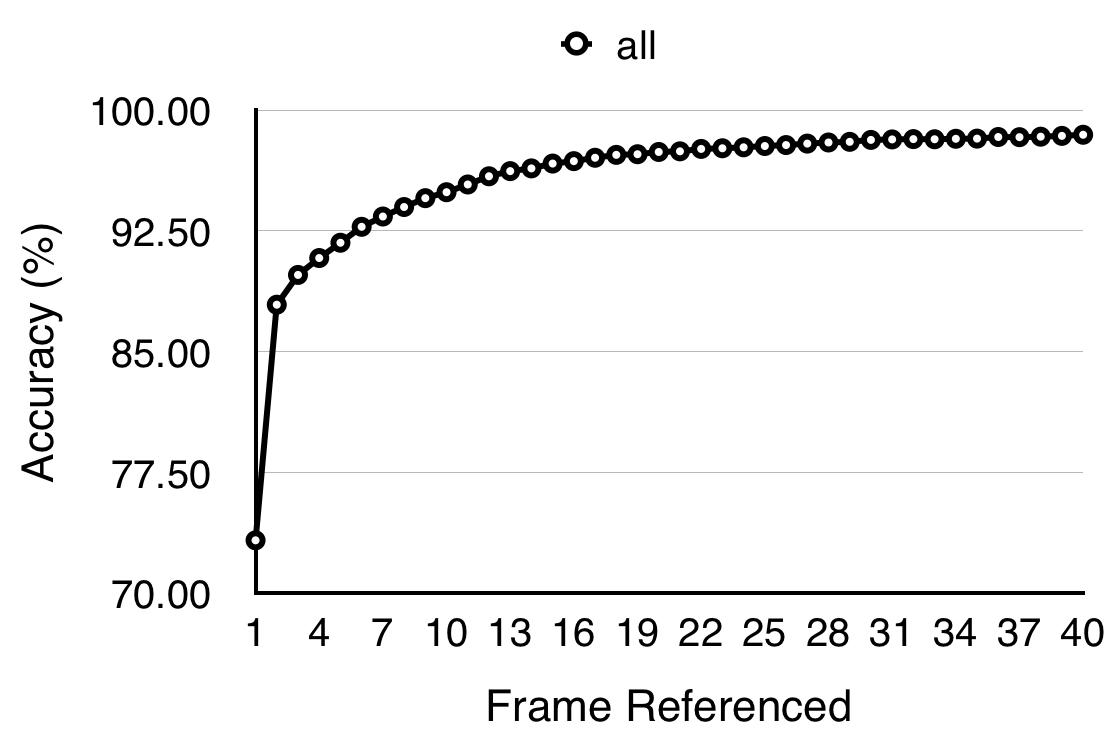
\includegraphics[width=1\columnwidth]{figures/figure3.png}
\caption{Classification accuracy of 5-fold cross validation for each user and leave-one-user-out cross validation. X axis is number of frame referenced while building Motion Signature ($N_{f}$) }
\label{fig:figure3}
\end{figure}


\subsection{Performance}
We ran a 5-fold cross validation with each participant's own data with parameters shown above. The averaged overall recognition rate is 98.83\%, with maximum 99.52\% and minimum 96.91\%.
We also conducted a leave-one-user-out cross validation, the averaged overall recognition rate is 83.71\%, with maximum 94.62\% and minimum 49.53\%.
Accuracy of leave-one-user-out cross validation strongly depends on users' behavior. If a user's behavior is very similar to another one, his/her accuracy will be relatively higher.
When we built a shared classifier with all participant's data, the performance was 98.42\% recognition rate in a 5-fold cross validation.
The confusion matrix of the shared classifier is shown at Table~\ref{tab:table1}.

\begin{table}
  \centering
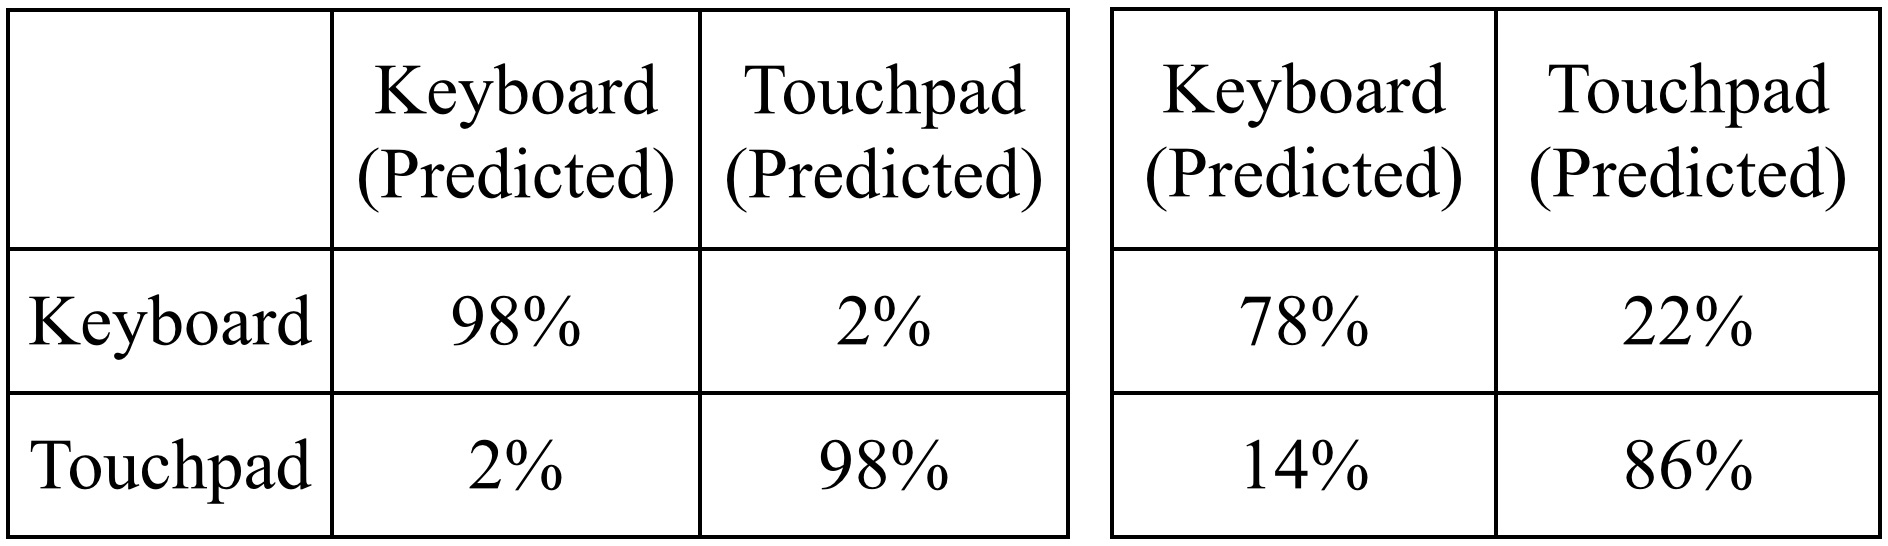
\includegraphics[width=1\columnwidth]{figures/confusion.jpg}
  \caption{Confusion matrix in a 5-fold cross validation(left) and leave-one-user-out cross validation(right)}
  \label{tab:table1}
\end{table}